\section{Synchronous Distributed Systems}
\label{chap:3}

In this model, processes partition the execution of algorithms into rounds. In each round, a processor can send messages, receive messages and perform some local computation. Synchronous systems come with guarantees properties on the nature of the system. For instance, upper bound on message delivery, ordered messages delivery, globally synchronised clocks, lock step based execution among others. 

Although it is difficult to implement a model with these strong assumptions, it is favourable for designing algorithms. The main problem with asynchronous systems is that message delay is unbounded, there is no limit on how long a process should wait in order to determine that it received all messages from its neighbours. Once an algorithm is designed for the synchronous model, it can be simulated in a more realistic model like an asynchronous system \cite{attiya2004distributed}.
% The reason why synchronous algorithms are desirable is that there are usually simpler to design and superior in complexity.

A synchronizer is a general technique to simulate synchronous communication in asynchronous systems. Synchronizer were introduced by Awerbuch \cite{awerbuch1985complexity}. The author presented 3 different synchronizers and analysed the trade off among them. This technique allows the execution of distributed synchronous algorithm over an asynchronous system, for instance, an asynchronous message passing system.  

The graphic \ref{fig:simulation} shows the interactions among the layers of the simulation. The bottom layer is the asynchronous message passing system, at this layer, there is no guarantees on messages delay. A synchronizer works on the top of this layer and its goal is to provide the illusion of a synchronous system to the upper layer. In the example, the user of the synchronizer is the Maximal Independent Set algorithm. Any user of the synchronizer can use the interface \textit{Sync-}$send_i$ and \textit{Sync-}$recv_i$ of the Synchronizer and safely assume that the communication is synchronous.     

\begin{figure}[ht]
\centering
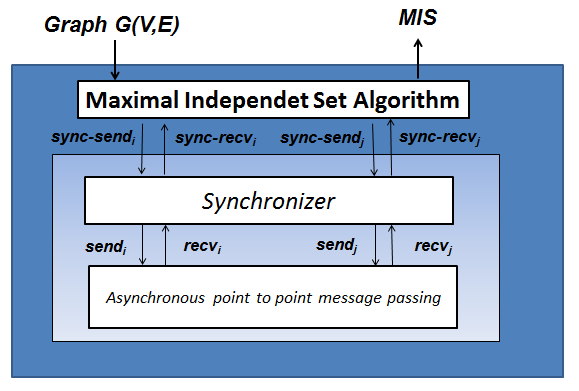
\includegraphics[width=1 \linewidth, height=8cm]{simulation.PNG} 
\caption{Diagram of the simulation of a synchronous distributed systems using synchronizers}
\label{fig:simulation}
\end{figure}



The following model was used in the original paper by Awerbuch \cite{awerbuch1985complexity} and was previously used in \cite{segall1983distributed,gallager1982distributed} among others. The asynchronous system is represented by an undirected graph $G = (V,E)$ where $V$ is the set of processes and $E$ is the set of bi-directional communication channels. The local model is also used for the synchronizer implementation. The messages delay is assumed to be finite in order to start a new round but there is no restriction on how long should be this delay. Another important assumption of the model is that the amount of information carried by messages is limited. 

Processes send messages after they receive a pulse or clock in the synchronous model. This pulse represents one time unit (round) in the synchronous system. The delay of the messages in one round is one unit of time of the global clock.

\begin{definition}
\label{def:safe}
A process $p_i$ is said to be safe in a round only after all its messages has been delivered at their destinations.
\end{definition}

The notion of safe process was introduced in \cite{awerbuch1985complexity}. If all neighbours of $p_i$ are safe for the round $r$, this mean that $p_i$ has received all messages for $r$. In this case, $p_i$ in ready to execute the $r + 1$ round. This property ensures that from the point of view of the user of the synchronizer, the network behaves as a synchronous communication system when it is really an asynchronous system. An easy solution to detect if a process is safe, it is to force each process to acknowledge every message that receives. 

The  overhead generated by a Synchronizer $S$ with the acknowledgement mechanism is the double the number of messages of the original algorithm $A$. To compute the total message and time complexity of a synchronous algorithm it is necessary to sum the complexity of $A$ and $S$. $T(S)$ and $M(S)$ denote the time and message complexity per round respectively. If the synchronizer requires an initialization phase (for instance, the Beta synchronizer) $T_{init}(S)$ and $M_{init}(S)$ express the message and time complexity for the initialization phase.  $M(A)$ and $T(A)$ are  the time and message complexity of the algorithm $A$. For algorithm implemented over a synchronizer, the total message complexity is then expressed in the equation \ref{ec:mess} and the time complexity in the equation \ref{ec:time}. 


\begin{equation}
\label{ec:mess}
 T_{tot} = T_{init}(S) + T(A)(1+T(S)) 
\end{equation}

\begin{equation}
\label{ec:time}
M_{tot} = M_{init}(S) + M(A) + T(A)M(S) 
\end{equation}


The two synchronizers presented in the next section are denoted Synchronizer $\alpha$ and Synchronizer $\beta$ \cite{awerbuch1985complexity}, which are a generalisation of the implementation proposed by Gallager in \cite{gallager1982distributed}. These two synchronizers present a trade off between messages and time complexity. Synchronizer $\alpha$ is efficient in time but produce a significant overhead in messages, while Synchronizer $\beta$ has a better performance in communication but it is worse in time complexity.



\subsection{Alpha Synchronizer}

One design challenge with synchronizers is the unbounded messages delay on real time. In consequence, a process cannot detect when it is safe just waiting until receiving all messages. The Alpha synchronizer use the acknowledgement mechanism to solve this problem. 

In the Synchronizer $\alpha$, a process $p_i$ send an acknowledgement for each message that receives. After $p_i$ has received all acknowledgement messages from its neighbour, $p_i$ knows that it is safe with respect to the round $r$. When $p_i$ detect that it's safe, then send a message \textbf{<safe,round>} to all its neighbours. Only after $p_i$ learns that all its neighbours are safe can start a new round.

The code for Synchronizer $\alpha$ is described in the algorithm \ref{algorithm:alpha}. The pseudo--code was extracted from \cite{attiya2004distributed}.  



\begin{algorithm}
 \caption{Alpha Synchronizer, code for $p_i$ from $i = 1$ to $N$}
 \label{algorithm:alpha} 

\SetAlgoNoLine

Initially \textit{round} = 0 and \newline
\textit{buffer[r], safe[r]} and \textit{ack-missing[r]} are empty for all $r \geq 1$ \newline

\textbf{When} \textit{Synch-}$send_i$ (S) occurs:\newline
$round = round + 1$ \newline
\textit{ack-missing[round]} = {$j:p_j$ is a recipient of a message in S} \newline
enable \textit{Asynch-}$send_i(<m,round>)$  to $p_j$, for each $m \in S$ with recipient $p_j$ \newline

\textbf{When} \textit{Asynch-}$recv_i(<ack,r>)$ from $p_j$ occurs: \newline
add $(m,j)$ to \textit{buffer[r]} \newline
enable $Asynch-send_i(<ack,r>)$ to $p_j$ \newline

\textbf{When} \textit{Asynch-}$recv_i(<ack,r>)$ from $p_j$ occurs: \newline
remove \textit{j} from \textit{ack-missing[r]} \newline
\If{ack-missing[r] = 0}{ 
enable \textit{Asynch-}$send_i(<safe,r>)$ to all neighbours \newline
}

\textbf{When} \textit{Asynch-}$recv_i(<safe,r>)$ from $p_j$ occurs: \newline
add \textit{j} to \textit{safe[r]} \newline
\If{safe[r] includes all neighbours}{
  enable \textit{Synch-}$recv_i(buffer[r])$ \newline
}

\end{algorithm}


In each round $p_i$ send extra messages to each neighbour, the equation \ref{ec:message-alpha} describe the message complexity of Synchronizer $\alpha$ per round.  For this synchronizer, $p_i$ needs one additional time unit in order to detect that it is safe, therefore the time complexity is constant, see equation \ref{ec:time-alpha}.  


\begin{equation}
\label{ec:message-alpha}
 C(\alpha) = O(E) = O(V^2) 
\end{equation}

\begin{equation}
\label{ec:time-alpha}
 T(\alpha) = O(1) 
\end{equation}


\subsection{Beta Synchronizer}

The Synchronizer $\beta$ is similar to the previous synchronizer. The difference with the Synchronizer $\alpha$ is the safe detection mechanism. This synchronizer needs an initialisation phase in which a rooted spanning tree is constructed over the network topology. A leader $S$ has to be chosen and then the spanning tree is constructed from the root. The acknowledgement mechanism is the same but instead of informs all its neighbours, $p_i$ just send the safe message to the parent in the spanning tree, this process is call convercast. A process $p_i$ is safe when has received the acknowledgement for each message sent in the actual round plus an additional \textbf{<safe,round>} from all its children in the spanning tree. Initially only processes that are on the bottom of the spanning tree (the leaves) send the message \textbf{<safe,round>} and progressively the parents of the leaves send this message to their parents once they are safe. When the root is safe, then broadcast \textbf{OK} on the spanning tree and every process is allowed to pursue with the next round. This blow up the time overhead since the mechanism acts as a global synchronizer with a central leader, which is the process acting as the root of the spanning tree. However, $p_i$ only send one safe message instead of sending to all its neighbourhood improving the message overhead of Alpha. 


\begin{algorithm}
 \caption{Beta Synchronizer, code for $p_i$ from $i = 1$ to $N$}
 \label{algorithm:beta} 

\SetAlgoNoLine

Compute a rooted spanning tree
Initially \textit{round} = 0 and \newline
\textit{buffer[r], safe[r]} and \textit{ack-missing[r]} are empty for all $r \geq 1$ \newline

\textbf{When} \textit{Synch-}$send_i$ (S) occurs:\newline
$round = round + 1$ \newline
\textit{ack-missing[round]} = {$j:p_j$ is a recipient of a message in S} \newline
enable \textit{Asynch-}$send_i(<m,round>)$  to $p_j$, for each $m \in S$ with recipient $p_j$ \newline

\textbf{When} \textit{Asynch-}$recv_i(<ack,r>)$ from $p_j$ occurs: \newline
add $(m,j)$ to \textit{buffer[r]} \newline
enable-$Asynch-send_i(<ack,r>)$ to $p_j$ \newline

\textbf{When} \textit{Asynch-}$recv_i(<ack,r>)$ from $p_j$ occurs: \newline
remove \textit{j} from \textit{ack-missing[r]} \newline
\If{ack-missing[r] = 0}{ 
enable \textit{Asynch-}$send_i(<safe,r>)$ to my parent in the spanning tree \newline
}
\If{$p_i$ is the root}{ 
enable \textit{Asynch-}$send_i(<go,r>)$ all my childrens in the spanning tree \newline
}

\textbf{When} \textit{Asynch-}$recv_i(<go,r>)$ from $p_j$ occurs: \newline
  enable \textit{Synch-}$recv_i(buffer[r])$ \newline
  enable \textit{Asynch-}$send_i(<go,r>)$ all my childrens in the spanning tree \newline

\end{algorithm}

The diameter of the spanning tree is $N - 1$, so the convercast and broadcast take at most $2N - 2$ time units combined. Time and message  complexity per synchronous round are expressed in the equations \ref{ec:message-beta} and \ref{ec:time-beta} respectively. The initialisation phase only needs to be done one time for each topology, for this reason it is more interesting the overhead $T(\beta)$ and $M(\beta)$. The time and message complexity of the initialization phase are $T_{init}(\beta) = O(V)$ and $M_{init}(\beta) = O(M + N \log N)$  respectively.

\begin{equation}
\label{ec:message-beta}
 C(\beta) = O(V)
 \end{equation}

\begin{equation}
\label{ec:time-beta}
 T(\beta) = O(V) 
\end{equation}

\subsection{Discussion about Synchronisation techniques}

One synchronizer is efficient in terms of time and the other in term of messages. The same author proposes \cite{awerbuch1985complexity} another synchronizer that tries to get a low overhead in both, the Synchronizer $\gamma$. Essentially, the idea is to generate a spanning forest of the graph and run Beta within each tree and Alpha between trees. If there are not too many adjacent trees, the messages overhead is similar to the Beta Synchronizer. The time overhead is proportional to the depth of the trees. In some special cases  (depending on the topology of the graph, for instance, a ring of k-cliques \cite{lynch1996distributed}), the Gamma Synchronizer can present a similar cost to the original synchronous algorithm. However, it is also possible the need of tune the spanning forest for some types of graphs. Besides, the Gama Synchronizer is more complex in terms of implementation and initialization phase.

All these synchronizers require that the entire network participate in the synchronization process, even if some processes have no message for some round. The problem is when $p_i$ do not send any messages in one round, then any process $p_j$ that is a neighbour of $p_i$ cannot deduce this situation because the delays in asynchronous networks are unbounded, in consequence, the use of timers are not useful. One solution is  to send dummy message in order to keep the synchronization. As a result, the overhead is always linear on the number of processes. Awerbuch and Peleg proposed in \cite{awerbuch1990network} a poly-logarithmic overhead synchronizer based on involving only the relevant portion of the topology in the synchronization process. However, it is possible that the synchronizer requires high space complexity.  Another approach for dynamic networks can rely on compute for each process the actives neighbours in every round and apply a simple synchronizer, Alpha for instance. This approach study in \cite{AspnesW2007} requires that each $p_i$ computes all neighbours before the execution of each round.

For the simulations in this project, besides the Beta and Alpha Synchronizers, another global synchronization mechanism is used. A master process $M$ is required to control the synchronization between every active process on the network.  Each process must inform $M$ that has finished the computation for the round $r$ and then $M$ is in charge of notifying active processes that are allow to start the $r + 1$ round. This mechanism generates a lot of computation in the master process, however, no unnecessary message is sent by inactive process. 

In the case of the Distributed Maximal Independent Set problem, especially with the algorithms explained in this chapter, this behaviour is desirable because many processes become inactive very quickly. These three techniques are used to simulate a synchronous communication for the \textit{MIS} algorithm. The analysis of the trade-off among them is presented in section \ref{chap:6}.




